%
% $RCSfile: wrapper.tex,v $
%
% Copyright (C) 2002-2008. Christian Heller.
%
% Permission is granted to copy, distribute and/or modify this document
% under the terms of the GNU Free Documentation License, Version 1.1 or
% any later version published by the Free Software Foundation; with no
% Invariant Sections, with no Front-Cover Texts and with no Back-Cover
% Texts. A copy of the license is included in the section entitled
% "GNU Free Documentation License".
%
% http://www.cybop.net
% - Cybernetics Oriented Programming -
%
% http://www.resmedicinae.org
% - Information in Medicine -
%
% Version: $Revision: 1.1 $ $Date: 2008-08-19 20:41:09 $ $Author: christian $
% Authors: Christian Heller <christian.heller@tuxtax.de>
%

\subsubsection{Wrapper}
\label{wrapper_heading}
\index{Wrapper Pattern}
\index{Adapter Pattern}
\index{Delegation Pattern}

The \emph{Wrapper} pattern \cite{gamma1995} allows otherwise incompatible
classes to work together. It can be seen as skin object enclosing (wrapping) an
inner core object, to which it provides access. In other words: It adapts the
interface of a class which is why Gamma et al. call the pattern \emph{Adapter}.
As can be seen in figure \ref{wrapper_figure}, this pattern makes heavy use of
\emph{Delegation}, where the \emph{Delegator} is the adapter (or wrapper) and
the \emph{Delegatee} is the class being adapted \cite{portland}.

\begin{figure}[ht]
    \begin{center}
        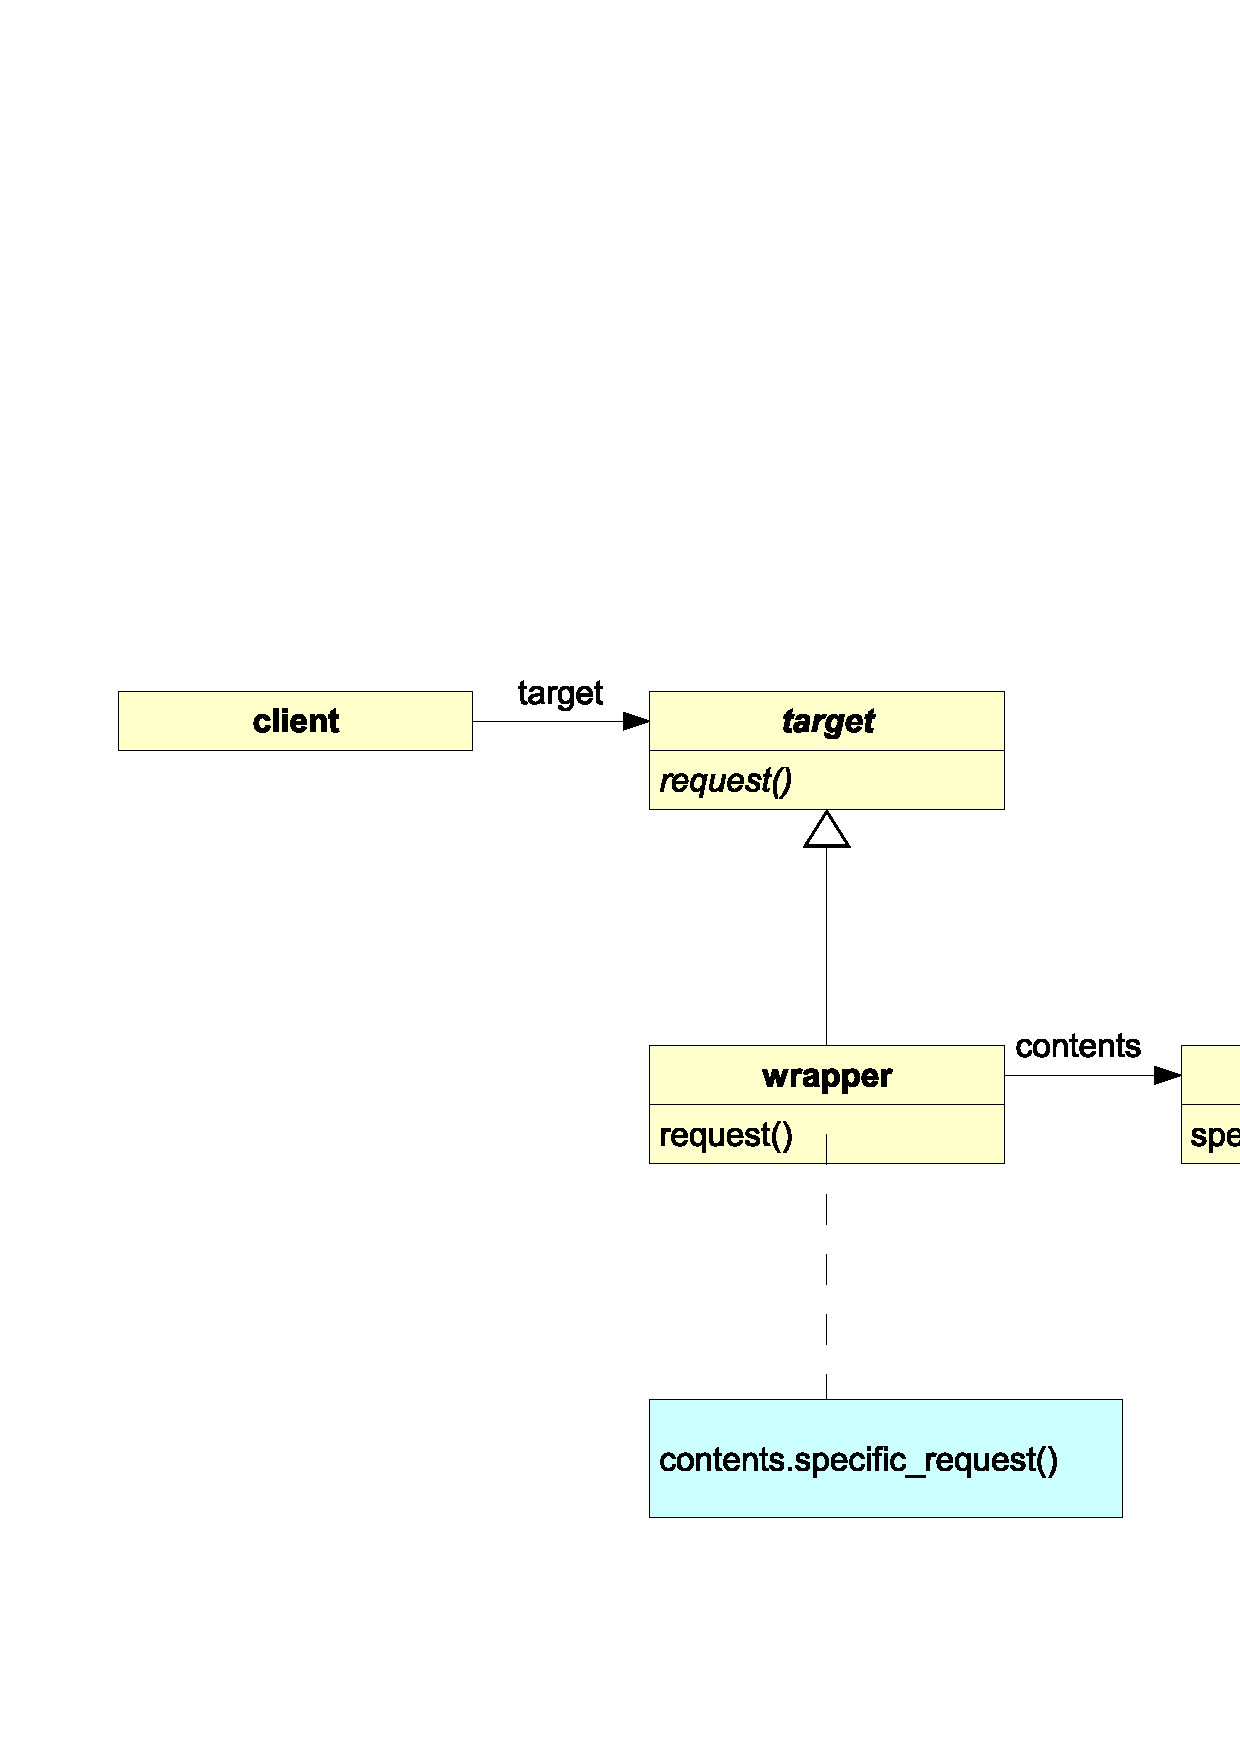
\includegraphics[scale=0.3,angle=-90]{graphic/wrapper.pdf}
        \caption{Wrapper Pattern}
        \label{wrapper_figure}
    \end{center}
\end{figure}

Knowledge templates created in the language described in chapter
\ref{cybernetics_oriented_language_heading} wrap the more fine-granular
templates they consist of.
